\documentclass[tikz,border=4pt]{standalone}
% Shared standard for all TikZ explainer figures (include after \documentclass[tikz,border=6pt]{standalone}).
% Rules: final width 16.5 cm (= \linewidth, scale 1.0); body text 8 pt, labels >= 7 pt, never smaller;
% every arrow starts/ends on a node anchor (never floats over text); edge labels use `fill=white` or sit
% above/below the arrow with at least 2 mm clearance; every box has inner sep >= 4 pt and its text fits
% inside (use text width / align=left / manual line breaks, then check the render); >= 5 mm gap between boxes;
% >= 4 mm padding between content and panel border; one accent colour per meaning (garnet = mismatch/bug).
\usepackage{fontspec}
\setmainfont{Liberation Serif}
\setsansfont{Liberation Sans}
\setmonofont[Scale=0.9]{Liberation Mono}
\renewcommand{\familydefault}{\sfdefault}% figure labels in sans; code chips stay mono
\usepackage{fontawesome5}
\usetikzlibrary{positioning,arrows.meta,fit,backgrounds,calc,shapes.geometric,shapes.symbols,decorations.pathreplacing}
\definecolor{garnet}{HTML}{8F001A}\definecolor{ink}{HTML}{2D2D2C}
\definecolor{cblue}{HTML}{2B6CB0}\definecolor{corange}{HTML}{D9822B}\definecolor{cgreen}{HTML}{2F855A}
\definecolor{pblue}{HTML}{EAF1FA}\definecolor{porange}{HTML}{FCEFE1}\definecolor{pgreen}{HTML}{E6F3EC}
\definecolor{accent}{HTML}{0072B2}\definecolor{stepblue}{HTML}{0072B2}\definecolor{pgrey}{HTML}{F2F2F2}\definecolor{pgarnet}{HTML}{F7E6E9}\definecolor{rule}{HTML}{B8B8B8}
\tikzset{
  every node/.style={font=\footnotesize,text=ink},
  small/.style={font=\scriptsize},
  panel/.style={rounded corners=5pt,draw=rule,line width=.4pt,inner sep=7pt},
  box/.style={rounded corners=3pt,draw=ink!60,fill=white,line width=.5pt,inner sep=4.5pt,align=center,minimum height=6mm},
  bug/.style={box,draw=garnet,fill=pgarnet,text=garnet,line width=.8pt},
  ok/.style={box,draw=cgreen,fill=pgreen},
  arr/.style={-{Stealth[length=2.2mm,width=1.8mm]},line width=.7pt,draw=corange},
  lab/.style={font=\scriptsize\itshape,fill=white,inner sep=1.5pt,text=ink!80},
  title/.style={font=\footnotesize\bfseries,anchor=north west},
  % Step badge: filled accent disc with a white number (white on #0072B2 is 5.2:1).
  badge/.style={circle,fill=stepblue,text=white,font=\bfseries\fontsize{8}{8}\selectfont,
    inner sep=0pt,minimum size=4.4mm},
  stepbadge/.style={circle,fill=stepblue,text=white,font=\bfseries\fontsize{7}{7}\selectfont,
    inner sep=0pt,minimum size=3.5mm},
  % Role chips: baseline execution = blue, transformed variant = orange, neutral = grey.
  basechip/.style={rounded corners=2pt,draw=cblue,fill=pblue,line width=.5pt,inner sep=2.5pt,
    font=\ttfamily\fontsize{7}{8.5}\selectfont,align=center,minimum height=5mm},
  varchip/.style={rounded corners=2pt,draw=corange,fill=porange,line width=.5pt,inner sep=2.5pt,
    font=\ttfamily\fontsize{7}{8.5}\selectfont,align=center,minimum height=5mm},
}

% Inline step badge for panel titles: \stepnum{1}Original query
\newcommand{\stepnum}[1]{\tikz[baseline=0pt]\node[stepbadge,anchor=base](sn){#1};\enspace}


\definecolor{okgreen}{HTML}{1E5631}

\tikzset{
  dia/.style={
    diamond, draw=ink!60, fill=white, aspect=2.0,
    minimum width=1.4cm, inner sep=1pt,
    font=\bfseries\fontsize{8}{9}\selectfont, line width=0.75pt
  },
  pill/.style={
    rounded corners=7pt, minimum width=2.6cm, minimum height=0.72cm,
    font=\bfseries\fontsize{8}{9.5}\selectfont, line width=0.8pt
  },
  tierlab/.style={
    font=\itshape\fontsize{7.5}{9.5}\selectfont, text=ink!60,
    align=right, text width=1.45cm
  },
  busline/.style={ink!60, line width=0.8pt, line cap=round},
}

\newcommand{\Card}[7]{%
  % #1 left x, #2 fill, #3 node name, #4 title, #5 subtitle, #6 expression pair, #7 oracle
  \node[panel, fill=#2, minimum width=3.32cm, minimum height=3.5cm,
    anchor=south west, inner sep=0pt] (#3) at (#1,3.4) {};
  \node[anchor=north west, inner sep=0pt, font=\bfseries\fontsize{10}{12}\selectfont]
    at (#1+0.35,6.72) {#4};
  \node[anchor=north west, align=left, text width=2.62cm, inner sep=0pt,
    font=\itshape\fontsize{7.5}{9}\selectfont, text=ink!70]
    at (#1+0.35,6.28) {#5};
  \node[anchor=center, align=center, text width=2.62cm, inner sep=0pt,
    font=\fontsize{7.5}{10}\selectfont\ttfamily, text=ink]
    at (#1+1.66,5.32) {#6};
  \draw[rule, line width=0.5pt, dash pattern=on 2pt off 2pt]
    (#1+0.35,4.58) -- (#1+2.97,4.58);
  \node[anchor=center, align=center, text width=2.62cm, inner sep=0pt,
    font=\fontsize{8}{9.5}\selectfont, text=ink]
    at (#1+1.66,3.92) {#7};
}

\begin{document}
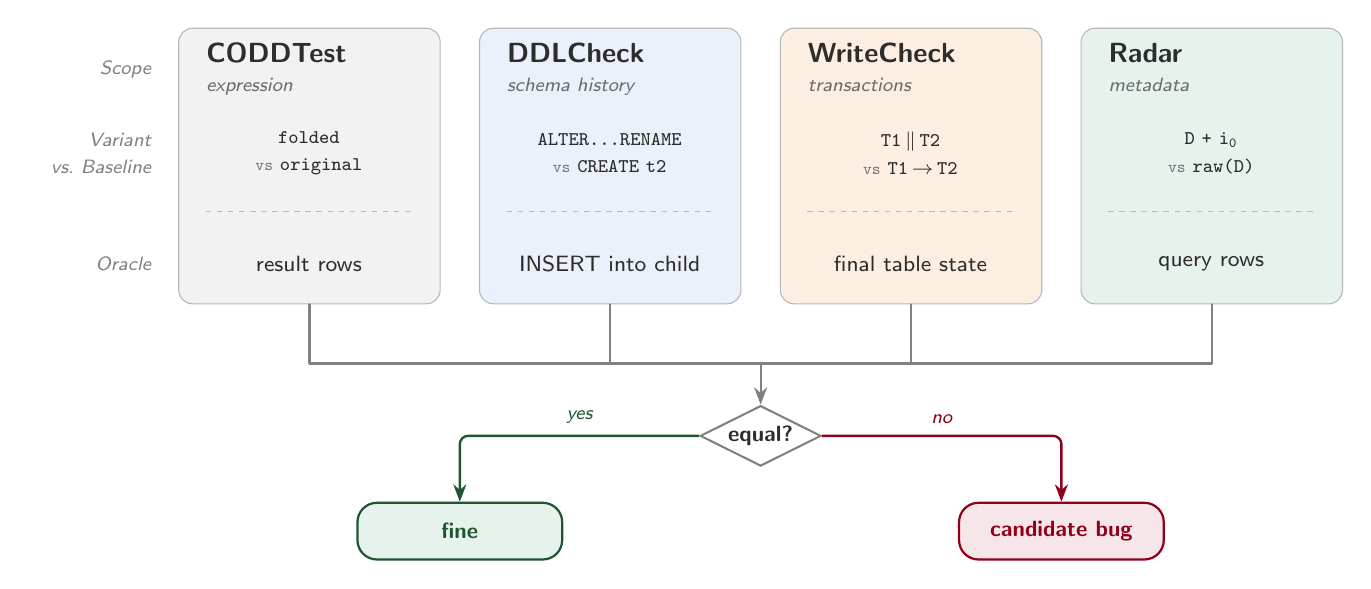
\begin{tikzpicture}[font=\fontsize{7.5}{9}\selectfont, text=ink]
  \node[tierlab, anchor=east] at (1.48,6.38) {Scope};
  \node[tierlab, anchor=east] at (1.48,5.32) {Variant\\vs.\ Baseline};
  \node[tierlab, anchor=east] at (1.48,3.92) {Oracle};

  % four cards: x0=1.7, pitch 3.82
  \Card{1.70}{pgrey}{cA}{CODDTest}{expression}
    {folded\\{\fontsize{6.5}{8}\selectfont\color{ink!65}vs} original}
    {result rows}
  \Card{5.52}{pblue}{cB}{DDLCheck}{schema history}
    {ALTER...RENAME\\{\fontsize{6.5}{8}\selectfont\color{ink!65}vs} CREATE t2}
    {INSERT into child}
  \Card{9.34}{porange}{cC}{WriteCheck}{transactions}
    {T1\,$\parallel$\,T2\\{\fontsize{6.5}{8}\selectfont\color{ink!65}vs} T1\,$\rightarrow$\,T2}
    {final table state}
  \Card{13.16}{pgreen}{cD}{Radar}{metadata}
    {D + i\textsubscript{0}\\{\fontsize{6.5}{8}\selectfont\color{ink!65}vs} raw(D)}
    {query rows}

  % shared orthogonal collector bus (busM derived, symmetry locked)
  \coordinate (busL) at (cA.south |- 0,2.65);
  \coordinate (busR) at (cD.south |- 0,2.65);
  \coordinate (busM) at ($(busL)!0.5!(busR)$);

  \foreach \c in {cA,cB,cC,cD} {
    \draw[busline] (\c.south) -- (\c.south |- 0,2.65);
  }
  \draw[busline] (busL) -- (busR);

  % decision diamond + symmetric pills under the card-pair midpoints
  \node[dia] (eq) at ($(busM) - (0,0.92)$) {equal?};
  \draw[-{Stealth[length=2.2mm]}, busline] (busM) -- (eq.north);

  \coordinate (leftCol)  at ($(cA.south)!0.5!(cB.south)$);
  \coordinate (rightCol) at ($(cC.south)!0.5!(cD.south)$);

  \node[pill, draw=okgreen, fill=pgreen, text=okgreen] (fine)
    at (leftCol |- 0,0.52) {fine};
  \node[pill, draw=garnet, fill=pgarnet, text=garnet] (bug)
    at (rightCol |- 0,0.52) {candidate bug};

  \draw[-{Stealth[length=2.2mm]}, okgreen, line width=0.85pt, rounded corners=3pt]
    (eq.west) -| (fine.north);
  \draw[-{Stealth[length=2.2mm]}, garnet, line width=0.85pt, rounded corners=3pt]
    (eq.east) -| (bug.north);

  % Mathematically centered branch labels
  \node[anchor=south, font=\fontsize{7.5}{9}\selectfont\itshape, text=okgreen, yshift=1pt]
    at ($(eq.west)!0.5!(eq.west -| fine.north)$) {yes};
  \node[anchor=south, font=\fontsize{7.5}{9}\selectfont\itshape, text=garnet, yshift=1pt]
    at ($(eq.east)!0.5!(eq.east -| bug.north)$) {no};
\end{tikzpicture}
\end{document}
